\documentclass[12pt, a4paper]{report}
\usepackage{tikz}
\usetikzlibrary{positioning,shadows,arrows}

\begin{document}
\title{Homework 6}
\author{Chang Wang}
\date{\today}

\maketitle

\section{Shortest path problem.}
\subsection{Give a reasonably efficient dynamic programming algorithm for finding a shortest path between p1 and p2.}
Here I use $R_{B_{i}^{u}}^{B_{j}^{v}} (1 \leq i < j \leq k , 1 \leq u < v \leq n)$ denotes the shortest path from aperture $u$ on Barrier $i$ to aperture $v$ on Barrier $j$. \\
First, I introduce two virtual Barriers 0 and (k+1) which go through point $p_{1}$ and $p_{2}$ respectively, and are parallel to other Barriers. Then, the dynamic programming fomulation is:
\begin{center}
$R_{B_{0}^{p_{1}}}^{B_{k+1}^{p_{2}}} = min \{R_{B_{0}^{p_{1}}}^{B_{i}^{u}} + R_{B_{i}^{u}}^{B_{j}^{v}} + R_{B_{j}^{v}}^{B_{k+1}^{p_{2}}}\}$
\end{center}
This algorithm requires to compare each two apertures on two barriers, which time complexity is $O(n^{2})$. Then it computes the minimum one, the time complexity is $O(k)$. Finally the complexity is $O(n^{2})$.

\subsection{divide-and-conquer algorithm.}
I'm sorry Dr. Gupta, I could not solve this question. Could you please give me some explanation or clue to help me figure it out. Thanks!

\section{Consider the problem of merging two sorted list A(1..k) and B(1..m).}
\subsection{Give a decision tree for merging A and B in the case that k=7 and m=2.}

Due to the page layout, I could not exhibit the whole figure in one page, so I divided it into separated parts. In the following figures, which stand for the decision tree. Each circle denotes a comparison, and the leave are in the ellipses.
\\
There should be {\bf 36 leaves} in the decision tree.
\begin{center}
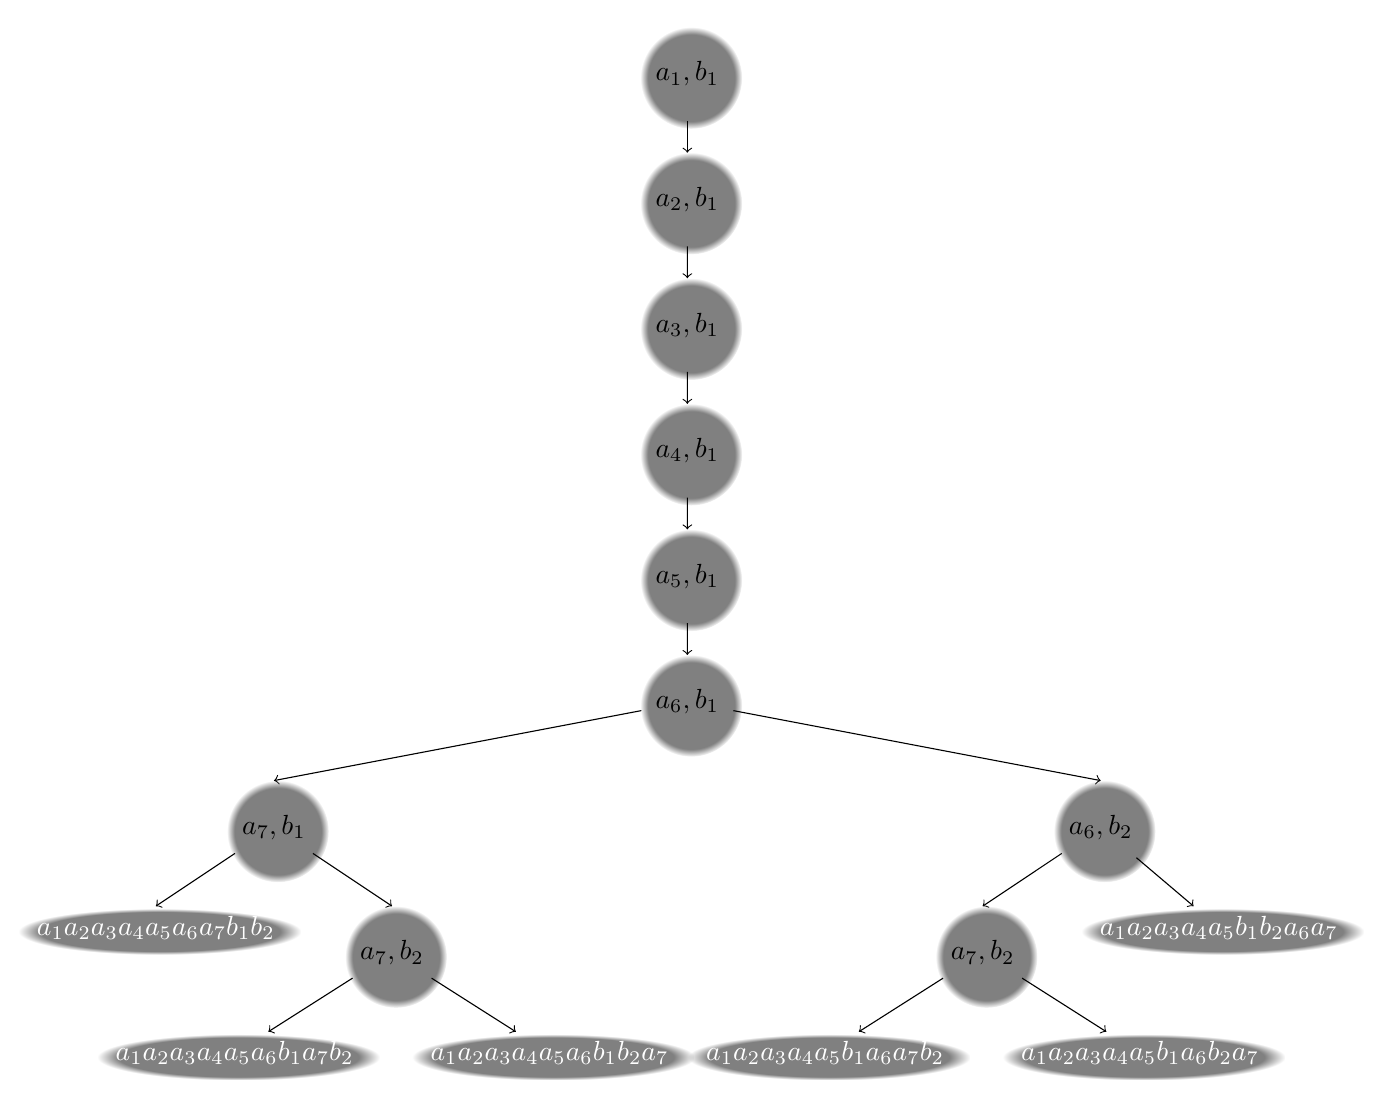
\begin{tikzpicture}[
		state/.style={circle, draw=none, text centered, anchor=north, text=black, circular drop shadow},
    leaf/.style={rectangle, draw=none, circular drop shadow,
        text centered, anchor=north, text=white},
    level distance=1cm, sibling distance=15cm
]

\node [state] (Root) {$a_{1}, b_{1}$} [->]
	child{ [sibling distance=12cm]
		node [state] {$a_{2}, b_{1}$}
		child {
			node [state] {$a_{3}, b_{1}$}
			child {
				node  [state]  {$a_{4}, b_{1}$}
				child {
					node  [state]  {$a_{5}, b_{1}$}
					child {  [sibling distance=10.5cm]
						node  [state]  {$a_{6}, b_{1}$}
						child {  [sibling distance=3cm]
							node  [state]  {$a_{7}, b_{1}$}
							child {  [sibling distance=4cm]
								node  [leaf]  {$a_{1}a_{2}a_{3}a_{4}a_{5}a_{6}a_{7}b_{1}b_{2}$}
							}
							child {  [sibling distance=4cm]
								node  [state]  {$a_{7}, b_{2}$}
								child { node  [leaf]  {$a_{1}a_{2}a_{3}a_{4}a_{5}a_{6}b_{1}a_{7}b_{2}$} }
								child { node  [leaf]  {$a_{1}a_{2}a_{3}a_{4}a_{5}a_{6}b_{1}b_{2}a_{7}$} }
							}
						}
						child {   [sibling distance=3cm]
							node  [state]  {$a_{6}, b_{2}$}
							child { [sibling distance=4cm]
								node [state] {$a_{7}, b_{2}$}
								child { node [leaf] {$a_{1}a_{2}a_{3}a_{4}a_{5}b_{1}a_{6}a_{7}b_{2}$} }
								child { node [leaf] {$a_{1}a_{2}a_{3}a_{4}a_{5}b_{1}a_{6}b_{2}a_{7}$} }
							}
							child { node [leaf] {$a_{1}a_{2}a_{3}a_{4}a_{5}b_{1}b_{2}a_{6}a_{7}$} }
						}
					}
				}
			}
		}
	}
;

\end{tikzpicture}
\end{center}

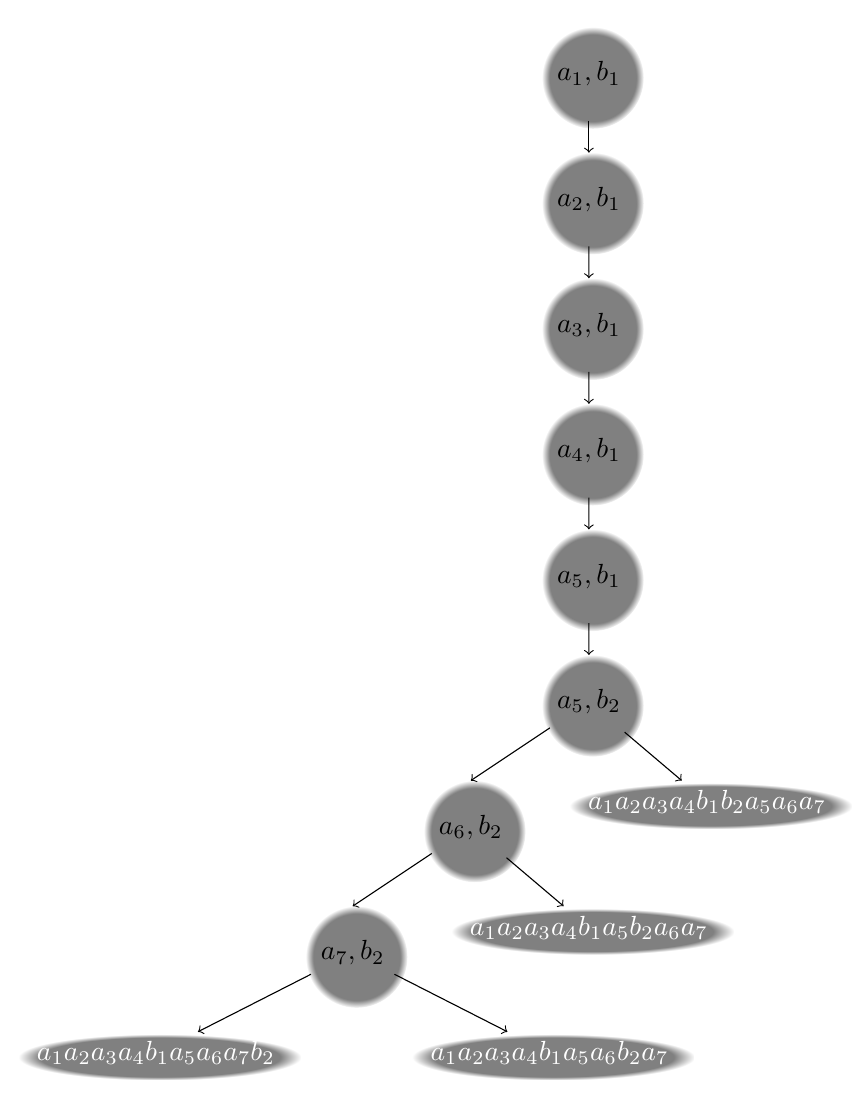
\begin{tikzpicture}[
		state/.style={circle, draw=none, text centered, anchor=north, text=black, circular drop shadow},
    leaf/.style={rectangle, draw=none, circular drop shadow,
        text centered, anchor=north, text=white},
    level distance=1cm, sibling distance=15cm
]

\node [state] (Root) {$a_{1}, b_{1}$} [->]
	child{ [sibling distance=12cm]
		node [state] {$a_{2}, b_{1}$}
		child {  [sibling distance=5cm]
			node [state] {$a_{3}, b_{1}$}
			child { [sibling distance=3cm]
				node  [state]  {$a_{4}, b_{1}$}
				child { [sibling distance=3cm]
					node  [state]  {$a_{5}, b_{1}$}
					child {  [sibling distance=3cm]
						node  [state]  {$a_{5}, b_{2}$}
						child {  [sibling distance=3cm]
							node  [state]  {$a_{6}, b_{2}$}
							child {   [sibling distance=5cm]
								node  [state]  {$a_{7}, b_{2}$} 
								child { node  [leaf]  {$a_{1}a_{2}a_{3}a_{4}b_{1}a_{5}a_{6}a_{7}b_{2}$} }
								child { node  [leaf]  {$a_{1}a_{2}a_{3}a_{4}b_{1}a_{5}a_{6}b_{2}a_{7}$} }
							}
							child { node  [leaf]  {$a_{1}a_{2}a_{3}a_{4}b_{1}a_{5}b_{2}a_{6}a_{7}$} }
						}
						child { node  [leaf]  {$a_{1}a_{2}a_{3}a_{4}b_{1}b_{2}a_{5}a_{6}a_{7}$} }
					}
				}
			}
		}
	}
;

\end{tikzpicture}

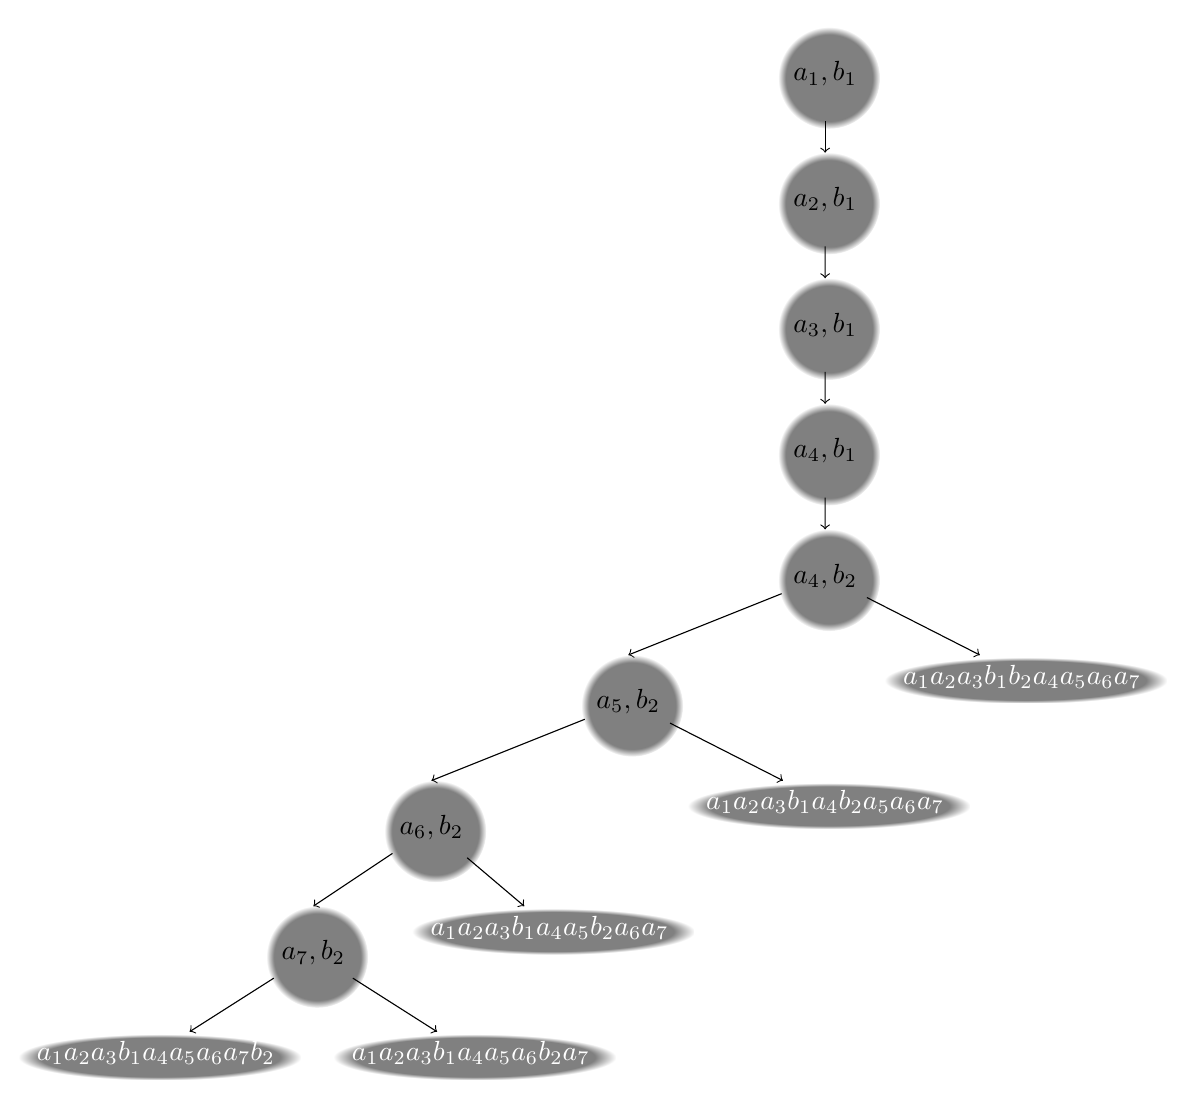
\begin{tikzpicture}[
		state/.style={circle, draw=none, text centered, anchor=north, text=black, circular drop shadow},
    leaf/.style={rectangle, draw=none, circular drop shadow,
        text centered, anchor=north, text=white},
    level distance=1cm, sibling distance=15cm
]

\node [state] (Root) {$a_{1}, b_{1}$} [->]
	child{
		node [state] {$a_{2}, b_{1}$}
		child { 
			node [state] {$a_{3}, b_{1}$}
			child {
				node  [state]  {$a_{4}, b_{1}$}
				child { [sibling distance=5cm]
					node  [state]  {$a_{4}, b_{2}$}
					child { [sibling distance=5cm]
						node  [state]  {$a_{5}, b_{2}$}
						child { [sibling distance=3cm]
							node  [state]  {$a_{6}, b_{2}$}
							child {  [sibling distance=4cm]
								node  [state]  {$a_{7}, b_{2}$}
								child { node  [leaf]  {$a_{1}a_{2}a_{3}b_{1}a_{4}a_{5}a_{6}a_{7}b_{2}$} }
								child { node  [leaf]  {$a_{1}a_{2}a_{3}b_{1}a_{4}a_{5}a_{6}b_{2}a_{7}$} }
							}
							child { node [leaf] {$a_{1}a_{2}a_{3}b_{1}a_{4}a_{5}b_{2}a_{6}a_{7}$} }
						}
						child { node  [leaf]  { $a_{1}a_{2}a_{3}b_{1}a_{4}b_{2}a_{5}a_{6}a_{7}$} }
					}
					child { node  [leaf]  { $a_{1}a_{2}a_{3}b_{1}b_{2}a_{4}a_{5}a_{6}a_{7}$} }
				}
			}
		}
	}
;

\end{tikzpicture}

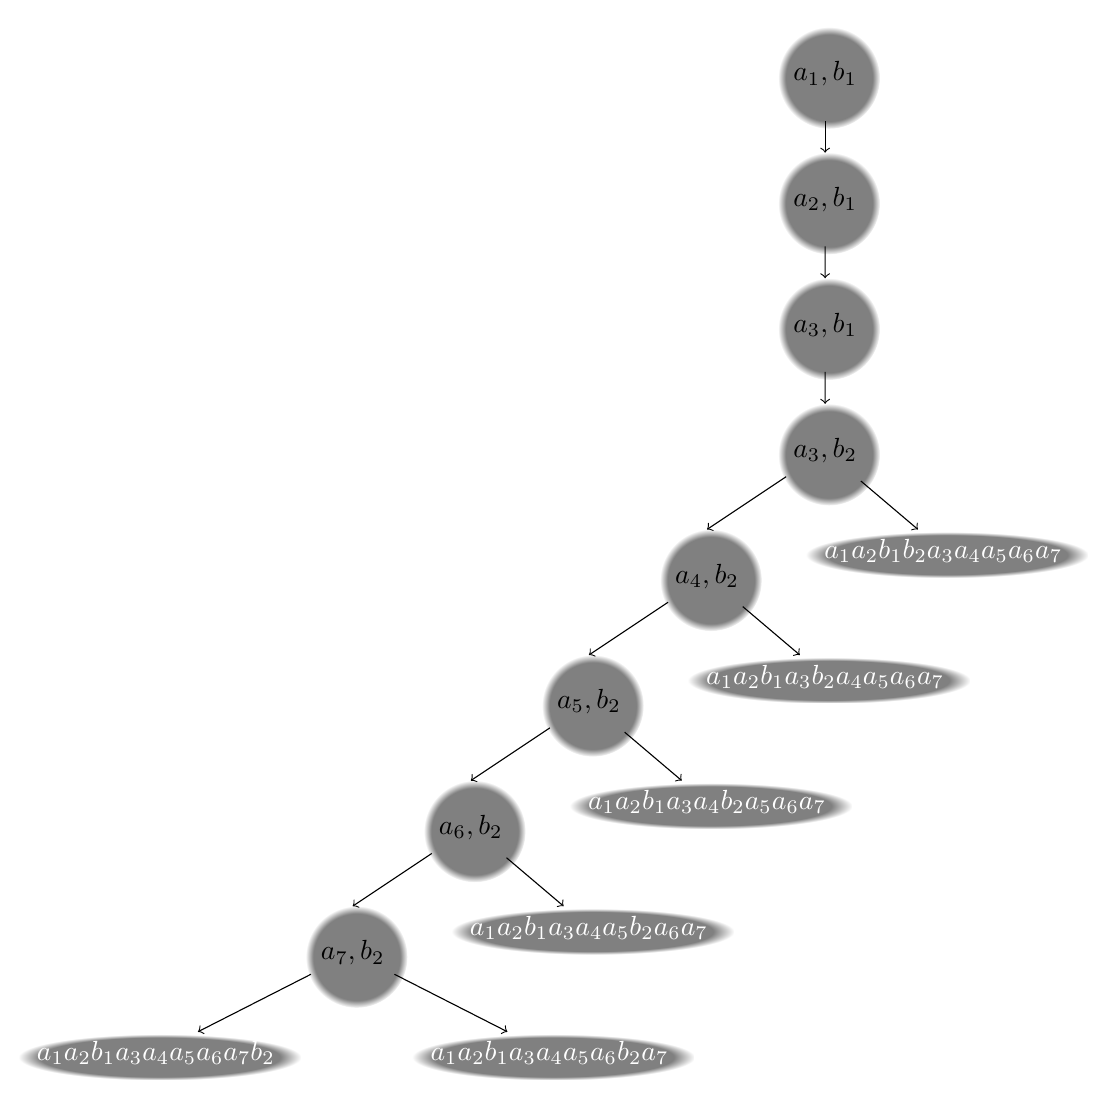
\begin{tikzpicture}[
		state/.style={circle, draw=none, text centered, anchor=north, text=black, circular drop shadow},
    leaf/.style={rectangle, draw=none, circular drop shadow,
        text centered, anchor=north, text=white},
    level distance=1cm, sibling distance=15cm
]

\node [state] (Root) {$a_{1}, b_{1}$} [->]
	child{ [sibling distance=12cm]
		node [state] {$a_{2}, b_{1}$}
		child {  [sibling distance=5cm]
			node [state] {$a_{3}, b_{1}$}
			child { [sibling distance=3cm]
				node  [state]  {$a_{3}, b_{2}$}
				child { [sibling distance=3cm]
					node  [state]  {$a_{4}, b_{2}$}
					child {  [sibling distance=3cm]
						node  [state]  {$a_{5}, b_{2}$}
						child {  [sibling distance=3cm]
							node  [state]  {$a_{6}, b_{2}$}
							child {   [sibling distance=5cm]
								node  [state]  {$a_{7}, b_{2}$} 
								child { node  [leaf]  {$a_{1}a_{2}b_{1}a_{3}a_{4}a_{5}a_{6}a_{7}b_{2}$} }
								child { node  [leaf]  {$a_{1}a_{2}b_{1}a_{3}a_{4}a_{5}a_{6}b_{2}a_{7}$} }
							}
							child { node  [leaf]  {$a_{1}a_{2}b_{1}a_{3}a_{4}a_{5}b_{2}a_{6}a_{7}$} }
						}
						child { node  [leaf]  {$a_{1}a_{2}b_{1}a_{3}a_{4}b_{2}a_{5}a_{6}a_{7}$} }
					}
					child { node  [leaf]  {$a_{1}a_{2}b_{1}a_{3}b_{2}a_{4}a_{5}a_{6}a_{7}$} }
				}
				child { node  [leaf]  {$a_{1}a_{2}b_{1}b_{2}a_{3}a_{4}a_{5}a_{6}a_{7}$} }
			}
		}
	}
;

\end{tikzpicture}

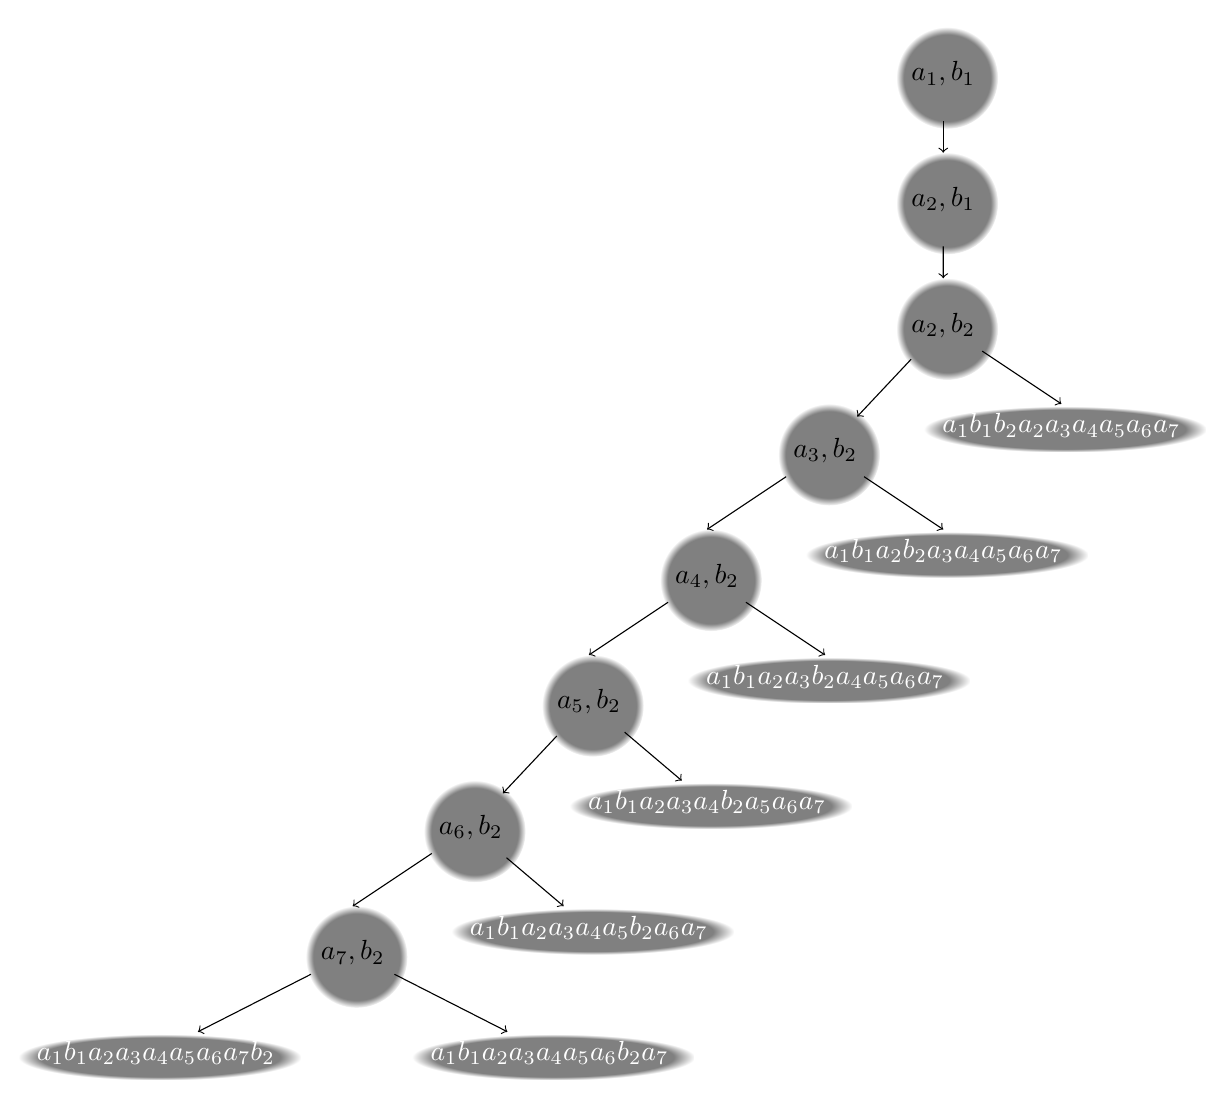
\begin{tikzpicture}[
		state/.style={circle, draw=none, text centered, anchor=north, text=black, circular drop shadow},
    leaf/.style={rectangle, draw=none, circular drop shadow,
        text centered, anchor=north, text=white},
    level distance=1cm, sibling distance=15cm
]

\node [state] (Root) {$a_{1}, b_{1}$} [->]
	child{ [sibling distance=12cm]
		node [state] {$a_{2}, b_{1}$}
		child {  [sibling distance=3cm]
			node [state] {$a_{2}, b_{2}$}
			child {
				node [state] {$a_{3}, b_{2}$}
				child { [sibling distance=3cm]
					node  [state]  {$a_{4}, b_{2}$}
					child { [sibling distance=3cm]
						node  [state]  {$a_{5}, b_{2}$}
						child {
							node  [state]  {$a_{6}, b_{2}$}
							child { [sibling distance=5cm]
								node  [state]  {$a_{7}, b_{2}$}
								child { node  [leaf]  {$a_{1}b_{1}a_{2}a_{3}a_{4}a_{5}a_{6}a_{7}b_{2}$} }
								child { node  [leaf]  {$a_{1}b_{1}a_{2}a_{3}a_{4}a_{5}a_{6}b_{2}a_{7}$} }
							}
							child { node  [leaf]  {$a_{1}b_{1}a_{2}a_{3}a_{4}a_{5}b_{2}a_{6}a_{7}$} }
						}
						child { node  [leaf]  {$a_{1}b_{1}a_{2}a_{3}a_{4}b_{2}a_{5}a_{6}a_{7}$} }
					}
					child { [sibling distance=4cm]
						node [leaf] {$a_{1}b_{1}a_{2}a_{3}b_{2}a_{4}a_{5}a_{6}a_{7}$}
					}
				}
				child { [sibling distance=4cm]
					node [leaf] {$a_{1}b_{1}a_{2}b_{2}a_{3}a_{4}a_{5}a_{6}a_{7}$}
				}
			}
			child { [sibling distance=4cm]
				node [leaf] {$a_{1}b_{1}b_{2}a_{2}a_{3}a_{4}a_{5}a_{6}a_{7}$}
			}
		}
	}
;

\end{tikzpicture}

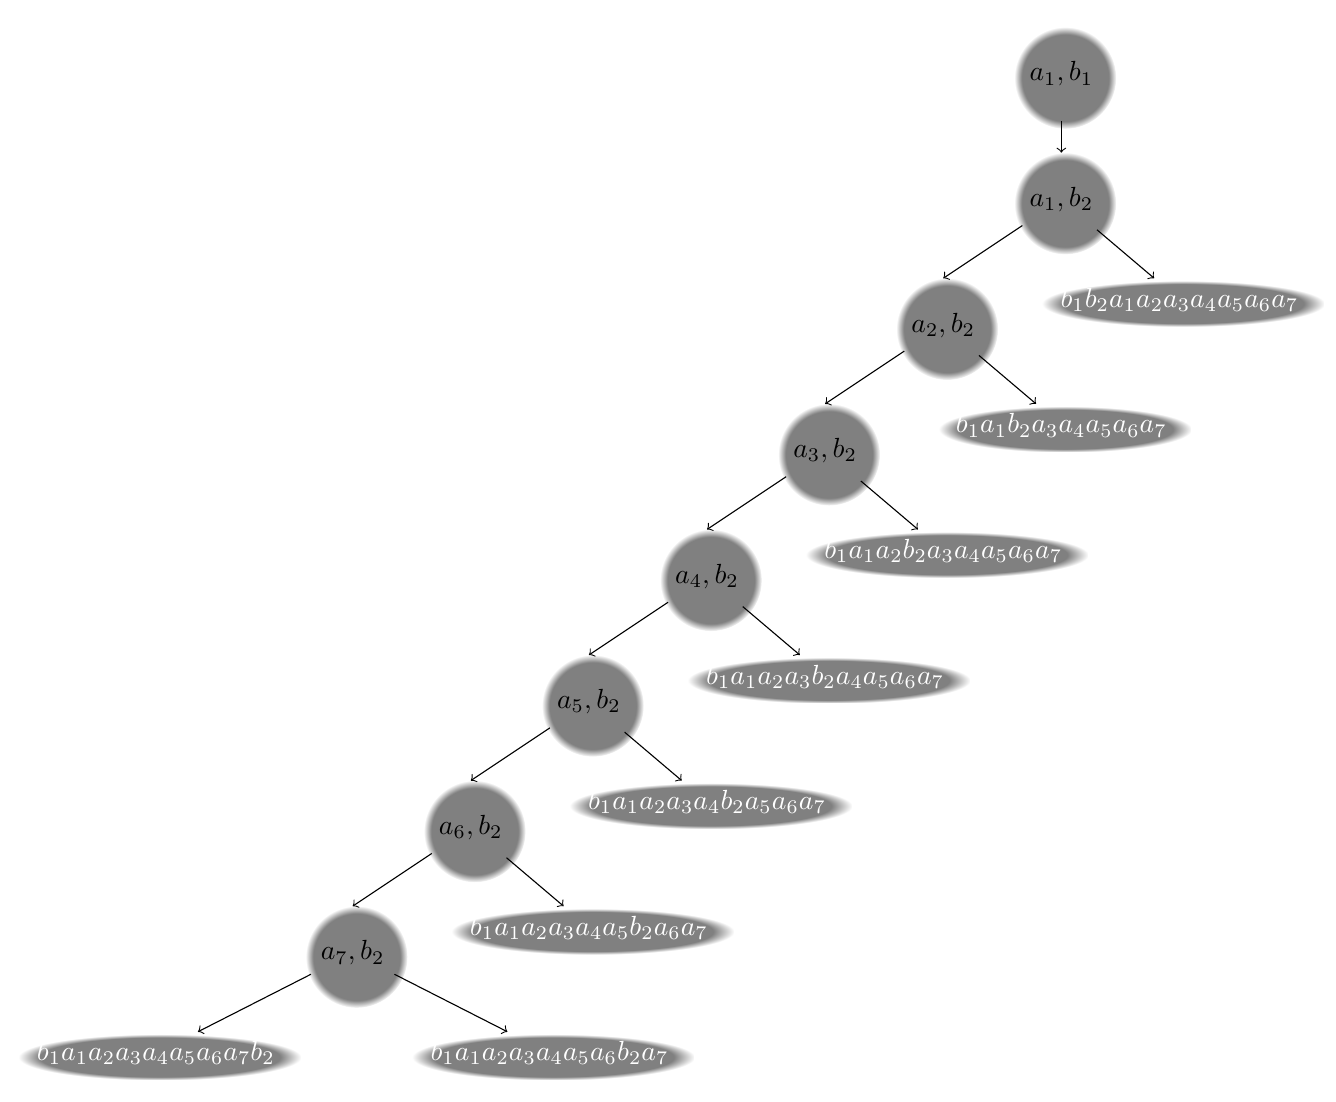
\begin{tikzpicture}[
		state/.style={circle, draw=none, text centered, anchor=north, text=black, circular drop shadow},
    leaf/.style={rectangle, draw=none, circular drop shadow,
        text centered, anchor=north, text=white},
    level distance=1cm, sibling distance=12cm
]

\node [state] (Root) {$a_{1}, b_{1}$} [->]
	child{  [sibling distance=3cm]
		node [state] {$a_{1}, b_{2}$}
		child {  [sibling distance=3cm]
			node [state] {$a_{2}, b_{2}$}
			child { [sibling distance=3cm]
				node  [state]  {$a_{3}, b_{2}$}
				child { [sibling distance=3cm]
					node  [state]  {$a_{4}, b_{2}$}
					child {  [sibling distance=3cm]
						node  [state]  {$a_{5}, b_{2}$}
						child {  [sibling distance=3cm]
							node  [state]  {$a_{6}, b_{2}$}
							child {  [sibling distance=5cm]
								node  [state]  {$a_{7}, b_{2}$}
								child { node  [leaf]  {$b_{1}a_{1}a_{2}a_{3}a_{4}a_{5}a_{6}a_{7}b_{2}$} }
								child { node  [leaf]  {$b_{1}a_{1}a_{2}a_{3}a_{4}a_{5}a_{6}b_{2}a_{7}$} }
							}
							child {
								node  [leaf]  {$b_{1}a_{1}a_{2}a_{3}a_{4}a_{5}b_{2}a_{6}a_{7}$}
							}
						}
						child {
							node  [leaf]  {$b_{1}a_{1}a_{2}a_{3}a_{4}b_{2}a_{5}a_{6}a_{7}$}
						}
					}
					child {
						node  [leaf]  {$b_{1}a_{1}a_{2}a_{3}b_{2}a_{4}a_{5}a_{6}a_{7}$}
					}
				}
				child { node  [leaf]  {$b_{1}a_{1}a_{2}b_{2}a_{3}a_{4}a_{5}a_{6}a_{7}$}
				}
			}
			child { node  [leaf]  {$b_{1}a_{1}b_{2}a_{3}a_{4}a_{5}a_{6}a_{7}$}
			}
		}
		child {   node  [leaf]  {$b_{1}b_{2}a_{1}a_{2}a_{3}a_{4}a_{5}a_{6}a_{7}$}
		}
	}
;

\end{tikzpicture}
\\[1cm]
\subsection{Find the number of leaves in a decision tree for merging A and B, assuming $k \geq m$.}

There are (k+m) elements in the final merged list, so it should have $(k+m)!$ possible permutations.  We divide it into two lists of length k and m respectively, then for each of the lists there are $k!$ and $m!$ possible permutations. Eventually, there are $k! \times m!$ total possible permutations. To find how many ways there are to divide $(k+m)$ numbers into 2 lists each size of n, divide total number of possible permutations of $(k+m)$ by total number of possible permutations of two lists of size k and m at the same time. 
\\
\begin{center}
$\frac{(k+m)!}{k!m!}$
\end{center}

And it also is the leaves in the decision tree for merging A and B.

\subsection{Using decision trees, give a lower bound on merging A and B, assuming $k \geq m$.}
Since each node in decision tree represents one comparison operation, the worst-case number of comparison for a merging is determined by the height of the tree. Lower bound on the tree height is the lower bound on the number of comparisons. For the simple sake, assume that all of the input elements are distinct, so we have a binary tree. Suppose the height of the tree is h, so this tree has no more than $2^{h}$ leaves. And we could get $2^{h} \geq \frac{(k+m)!}{k!m!}$, then we have $h \geq \log \frac{(k+m)!}{k!m!}$.\\[0.5cm]
$\frac{(k+m)!}{k!m!} = \frac{(k+m)(k+m-1)...(k+1)(k!)}{k!m!} = \frac{(k+m)(k+m-1)...(k+1)}{m(m-1)...1}$ \\[0.5cm]
Due to $k \geq m$, we could have $\frac{k+m}{m} \geq 2$. \\
So, above formula could be changed to $(\frac{k+m}{m}) (\frac{k+m-1}{m-1}) ... (\frac{k+1}{1}) \geq 2^{m}$ \\
Finally, $h \geq \log \frac{(k+m)!}{k!m!} \geq \log (2^{m}) \geq \Omega (m)$ \\
The lower bound on merging A and B is: $\Omega (m)$.
\end{document}  